% Created 2021-07-19 Mon 09:53
% Intended LaTeX compiler: pdflatex
\documentclass[presentation]{beamer}
\usepackage[utf8]{inputenc}
\usepackage[T1]{fontenc}
\usepackage{graphicx}
\usepackage{grffile}
\usepackage{longtable}
\usepackage{wrapfig}
\usepackage{rotating}
\usepackage[normalem]{ulem}
\usepackage{amsmath}
\usepackage{textcomp}
\usepackage{amssymb}
\usepackage{capt-of}
\usepackage{hyperref}
\usetheme{default}
\author{Jonathan Fairbanks}
\date{\today}
\title{Innovation week : Spring framework}
\hypersetup{
 pdfauthor={Jonathan Fairbanks},
 pdftitle={Innovation week : Spring framework},
 pdfkeywords={},
 pdfsubject={},
 pdfcreator={Emacs 27.1 (Org mode 9.5)}, 
 pdflang={English}}
\begin{document}

\maketitle
\begin{frame}{Outline}
\tableofcontents
\end{frame}

unorganized notes taken as I go.

\begin{frame}[label={sec:org34d6546}]{PluralSight}
\begin{block}{Java Spring}
\url{https://app.pluralsight.com/library/courses/spring-framework-spring-fundamentals/table-of-contents}
\begin{block}{What is Spring}
\begin{block}{Dependency Injection framework}
\end{block}
\end{block}
\begin{block}{Spring configuration using Java}
\begin{block}{@Beans}
decorator over methods

by default they are singletons meaning it will only be called once
\end{block}
\begin{block}{Setter injection}
\end{block}
\begin{block}{Constructor injection}
basically the same as setter except it's as constructor instead of a setter
\end{block}
\end{block}
\begin{block}{Scopes}
\begin{block}{Singleton}
\begin{block}{default bean scope}
\end{block}
\begin{block}{One instantiation}
\end{block}
\begin{block}{Single instance per Spring container}
\end{block}
\begin{block}{Added with @Scope over method}
\end{block}
\end{block}
\begin{block}{Prototype}
bean per request
\begin{block}{Per request}
\end{block}
\begin{block}{Garunteed Uniq}
\end{block}
\begin{block}{Added with @Prototype overmethod}
\end{block}
\end{block}
\begin{block}{Web aware}
\begin{block}{Request}
\end{block}
\begin{block}{Session}
\end{block}
\begin{block}{Global}
\end{block}
\end{block}
\end{block}
\begin{block}{Autowired}
Makes things a lot easier since you do not have to call any of the set/constructor injection for services, as long as everything has the appropriate decorators above them
\begin{block}{@ComponentScan(\{``''\}) <- look for inside quote}
\end{block}
\end{block}
\begin{block}{Stereotypes}
\begin{block}{@Component}
\end{block}
\begin{block}{@Repository}
\end{block}
\begin{block}{@Service}
\end{block}
\begin{block}{@Controller}
\end{block}
\end{block}
\begin{block}{Advanced Bean Configuration}
\begin{block}{Bean Lifecycle}
instantiation -> populate properties -> BeanNameAware -> BeanFactoryAware -> Pre initialization - BeanPostProcessors -> InitialaizeBean -> InitMethod -> Post init - BeanPostProcessors
\end{block}
\begin{block}{FactoryBean}
\begin{block}{What?}
\end{block}
\end{block}
\begin{block}{SpEL (Spring Expression Language)}
\begin{block}{Manipualte object Graph}
\end{block}
\begin{block}{Evaluate at runtime}
\end{block}
\begin{block}{Security}
@Value(``\#\{\}'') can be done run time which will be injected into code.
\end{block}
\end{block}
\begin{block}{Proxies}
\begin{block}{@Transactional}
\end{block}
\end{block}
\begin{block}{Profiles}
\begin{block}{Adapt Environments}
\end{block}
\begin{block}{Runtime Configuration}
\end{block}
\begin{block}{@Profile(``'')}
\end{block}
\begin{block}{Add into vm option}
-Dspring.profiles.active=profileName
\end{block}
\end{block}
\end{block}
\end{block}
\begin{block}{Java Spring JPA}
\begin{block}{Spring JPA}
\begin{block}{Enhances JPA}
\end{block}
\begin{block}{Simplifies Data Tier}
\end{block}
\begin{block}{JpaRepository}
\end{block}
\begin{block}{Query DSL}
\end{block}
\begin{block}{Data Tier}
\end{block}
\end{block}
\begin{block}{JPA (Java Persistence API)}
an object relation mapping - Relational tables <-> Software objects.
[Honestly sounds a lot like entity framework from .NET]
\end{block}
\begin{block}{JPA Repository}
A repository in the repositories folder that is an interface that extends from JPARepository. and that is it.
\begin{block}{Spring repositories themselves do not need to be an interface}
\end{block}
\begin{block}{DAO (Data Acess Object) focus}
\end{block}
\begin{block}{Are interfaces, not classes}
\end{block}
\begin{block}{map 1:1 with a JPA Entity}
\end{block}
\end{block}
\begin{block}{Architecure}
\href{./Resources/RepoArchitecture.png}{Repository Architecture}
code injection ->
\end{block}
\begin{block}{Decorators}
\begin{block}{@ID}
Pretty much the primary key of the data when represnted in tables on a DB
\begin{block}{GenerationType.}
\url{https://stackoverflow.com/questions/47676403/spring-generatedvalue-annotation-usage}
good stack overflow describing usage of each term
\begin{block}{Auto}
default and picks based on provider i.e hibernation -> sequence
\end{block}
\begin{block}{Identity}
uses DBs auto increment not good for hibernate since hibernate requires a primary key value for each entity.
\end{block}
\begin{block}{Sequence}
uses db unique but requires an additional select (almost no performance impact for most applications?)
\end{block}
\begin{block}{Table}
simulated sequence
\end{block}
\end{block}
\begin{block}{Database relationships}
You can specify where a part of an entity relates to another with JPA by adding decorators such as @ManyToOne @ManyToMany as such over parts of an object
\end{block}
\end{block}
\end{block}
\begin{block}{Seperation of Concerns}
\begin{block}{Presentation Layer}
\end{block}
\begin{block}{Business Logic}
\end{block}
\begin{block}{Data Layer}
\end{block}
\end{block}
\begin{block}{Components}
\begin{block}{Controller}
handles request, no business logic
coordinated with service and repository
\begin{block}{@Controller}
\end{block}
\end{block}
\begin{block}{Service}
business logic belongs here
transactional
often same methods as the repository. So things such as if the result from a repository is empty do X
described as the verbs of a system
\begin{block}{@Service}
\end{block}
\end{block}

\begin{block}{Repository}
Data Access Object usually 1:1 to table, described as the ``nouns'' of the system
\begin{block}{@Repository}
\end{block}
\end{block}
\end{block}
\begin{block}{Entity tagging}
\begin{block}{@Entity}
marks it as something that is tied into a database
\end{block}
\begin{block}{@Id}
marks what field is the primary key
\end{block}
\begin{block}{@GeneratedValue}
what type of primary key
\end{block}
\end{block}
\begin{block}{Database Creation Values}
spring.jpa.hibernate.ddl-auto=
\begin{block}{Create}
\end{block}
\begin{block}{Update}
\end{block}
\begin{block}{Create-drop}
\end{block}
\begin{block}{Validate}
\end{block}
\begin{block}{None}
\end{block}
\end{block}
\begin{block}{Application properties}
\begin{block}{Forced uppercase tables}
spring.jpa.hibernate.naming.physical-strategy=

org.hibernate.boot.model.naming.PhysicalNamingStrategyStandardImpl
\end{block}
\end{block}

\begin{block}{JPA Annotations}
\begin{block}{@Entity - Declares Object}
\end{block}
\begin{block}{@Table - Table specifics}
\end{block}
\begin{block}{@Id - Primary key}
\end{block}
\begin{block}{@GeneratedValue - Used with @Id}
\begin{block}{IDENTITY - Column}
\end{block}
\begin{block}{AUTO - Chooses from dialect}
\end{block}
\begin{block}{SEQUENCE - if database supports it}
\end{block}
\begin{block}{TABLE - uses identity table}
\end{block}
\end{block}
\begin{block}{@PresistenceContext - injects EntityManager}
\end{block}
\begin{block}{@Service - Location of business logic}
\end{block}
\begin{block}{@Repository - Database Integration}
\end{block}
\begin{block}{Transactional - Begining of Transaction}
\end{block}
\end{block}
\begin{block}{Default columns}
@Column
\begin{block}{insertable}
\end{block}
\begin{block}{length}
\end{block}
\begin{block}{name}
\end{block}
\begin{block}{nullable}
\end{block}
\begin{block}{precision}
\end{block}
\begin{block}{scale}
\end{block}
\begin{block}{table}
\end{block}
\begin{block}{unique}
\end{block}
\begin{block}{updatable}
\end{block}
\end{block}
\begin{block}{Join Types}
\begin{block}{@OneToOne}
\end{block}
\begin{block}{@OneToMany}
\end{block}
\begin{block}{@ManyToOne}
\end{block}
\begin{block}{@ManyToMany}
\end{block}
\end{block}
\begin{block}{FetchTypes}
\begin{block}{Lazy}
\end{block}
\begin{block}{Eager}
\end{block}
\end{block}
\begin{block}{JPQL}
centered around objects
ex:

Query q = em.createQuery(``Select r from Registration'');

where r is an object
\end{block}
\begin{block}{NamedQueries}
Cleaner but not required.
@NamedQueries(\{
    @NamedQuery(x=, y=)
\})
\end{block}
\begin{block}{Query DSL (Domain Specific Language)}
method contracts

\begin{block}{Begins with}
(examples from video there are more things you can have such as countBy or findFirstBy)
\begin{block}{findBy}
\end{block}
\begin{block}{queryBy}
\end{block}
\begin{block}{readBy}
\end{block}
\begin{block}{countBy}
\end{block}
\begin{block}{getBy}
\end{block}
\end{block}
\begin{block}{Uses JPA attributes names for criteria}
\end{block}
\begin{block}{Multiple criteria combined with ``And'', ``Or''}
\end{block}
\begin{block}{Default for DSL is to use = on a query}
to change that you must have Is, Equals or Not as part of the method
\end{block}
\begin{block}{Other comparisons}
\begin{block}{LessThan}
\end{block}
\begin{block}{LessThanEqual}
\end{block}
\begin{block}{GreaterThan}
\end{block}
\begin{block}{GreaterThanEqual}
\end{block}
\begin{block}{True}
\end{block}
\begin{block}{False}
\end{block}
\begin{block}{In}
\end{block}
\begin{block}{NotIn}
\end{block}
\begin{block}{IgnoreCase}
\end{block}
\begin{block}{OrderBy}
\end{block}
\begin{block}{First}
\end{block}
\begin{block}{TopX <- X is a number}
\end{block}
\begin{block}{Distinct}
\end{block}
\end{block}
\begin{block}{Date Comparisons}
no beforeEqual or afterEqual keywords
\begin{block}{Before(startDate)}
\end{block}
\begin{block}{After(startDate)}
\end{block}
\begin{block}{Between(startDate, endDate)}
\end{block}
\end{block}
\begin{block}{Null}
\begin{block}{Null}
\end{block}
\begin{block}{IsNull}
\end{block}
\begin{block}{NotNull}
\end{block}
\begin{block}{IsNotNull}
\end{block}
\end{block}
\end{block}
\begin{block}{@Query}
when you hand write your query
\begin{block}{good for specific joining (left, right joins)}
\end{block}
\begin{block}{eager loading control}
\end{block}

\begin{block}{It is possible to use NativeQuery with ``nativeQuery=true'' in the parameters for the query, but kind of locks you in (No JPQL)}
\end{block}
\begin{block}{NamedQuery}
queries that can be recalled elsewhere

@NamedQuery(
    name=``''
    query=``''
)
\end{block}
\end{block}
\end{block}

\begin{block}{Other notes}
\begin{block}{Keybinds}
\begin{block}{Ctrl + Shift + O}
removes unused imports
\end{block}
\end{block}
\begin{block}{PluralSight}
\begin{block}{Leaving the RequestMapping blank?}
\end{block}
\end{block}
\begin{block}{Why is it called @Lob}
-> stores binary data
\end{block}
\begin{block}{Acronym purgatory}
\begin{block}{JPA - Java Persistence API}
\end{block}
\begin{block}{EJB - Enterpise Java Bean}
\end{block}
\begin{block}{JNDI - Java Naming and Directory Interface}
\end{block}
\begin{block}{JEE - Java Enterpise Edition}
\end{block}
\begin{block}{POJO - Plain Old Java Object}
\end{block}
\begin{block}{AOP - Aspect oriented programming}
\end{block}
\begin{block}{ORM - Object Relational Mapping}
\end{block}
\begin{block}{Java Server Pages}
\end{block}
\end{block}
\begin{block}{Best practices}
\begin{block}{Singleton}
\end{block}
\begin{block}{Factories}
\end{block}
\begin{block}{Abstract Factories}
\end{block}
\begin{block}{Template Method}
\end{block}
\begin{block}{Annotation Based}
\end{block}
\end{block}
\end{block}
\end{frame}

\begin{frame}[label={sec:org346ba75}]{Spring.io Docs}
\begin{block}{Framework Reference}
\url{https://docs.spring.io/spring-framework/docs/3.2.x/spring-framework-reference/html/overview.html}
\begin{block}{Modules}
\begin{block}{Core container}
contains core, beans, context, and expression language modules
\begin{block}{Core \& Beans}
seperates configuration from dependecies
\end{block}
\begin{block}{Beans}
3 things
\begin{block}{Serializable}
\end{block}
\begin{block}{something}
\end{block}
\begin{block}{something}
\end{block}
\end{block}
\begin{block}{Context}
access objects similar to (JNDI registry)
\begin{block}{JNDI Registry}
\url{https://docs.oracle.com/javase/tutorial/jndi/overview/index.html}
Java Naming and Direcotry interface

it is an API that provides naming and directory functionality
\begin{center}
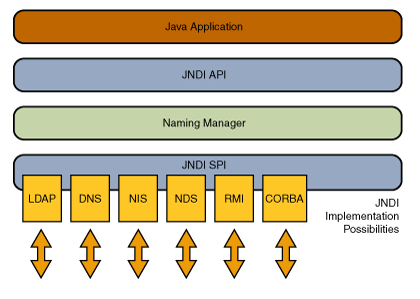
\includegraphics[width=.9\linewidth]{./Resources/JNDI.png}
\end{center}
\end{block}
\end{block}
\end{block}
\end{block}
\end{block}
\begin{block}{The IoC Container}
\url{https://docs.spring.io/spring-framework/docs/3.2.x/spring-framework-reference/html/beans.html}
(IoC) Inversion of Control which describes the process of a container injecting dependecies when creating beans
\begin{block}{Factory Method}
a design pattern that describes making objects at run time. (where all objects share the superclass)
\end{block}
\end{block}
\end{frame}
\begin{frame}[label={sec:orgbb65cb0}]{TutorialsPoint}
\end{frame}
\begin{frame}[label={sec:org0fcfc3b}]{MasterControl}
\begin{block}{Getter and Setter tags used on some entities}
\end{block}
\begin{block}{SLf4j}
\begin{block}{Stands for Simple Logging Facade for Java}
very easy to remember
\end{block}
\end{block}
\begin{block}{Table with schema parameter used a fair bit}
\end{block}
\end{frame}
\end{document}
